\section{Алгоритмы обхода графа в глубину и ширину.}

\begin{definition}
    Обход графа (поиск на графе) –- это процесс систематического просмотра
    всех ребер или вершин графа с целью отыскания ребер или вершин,
    удовлетворяющих некоторому условию.
\end{definition}

\begin{definition}
    Поиск в ширину (BFS) нужен для нахождения расстояний между вершин в связном графе.
    Алгоритм по принципу напоминает "пожар".
\end{definition}

Алгоритм поиска в ширину:
\begin{enumerate}[left=0.0em, labelsep=1em, topsep=0em, itemsep=0pt, parsep=0.5em]
    \item Все вершины окрашиваются в белый цвет.
    \item Выбирается первая вершина, раскрашивается в черный цвет и заносится в очередь.
    \item Посещается первая вершина из очереди. Все смежные с ней белые вершины
    раскрашиваются в черный цвет и заносятся в очередь. После этого эта вершина удаляется
    из очереди.
    \item Повторяется шаг 3 до тех пор пока очередь не пуста.
\end{enumerate}

\begin{figure}[h]
    \centering
    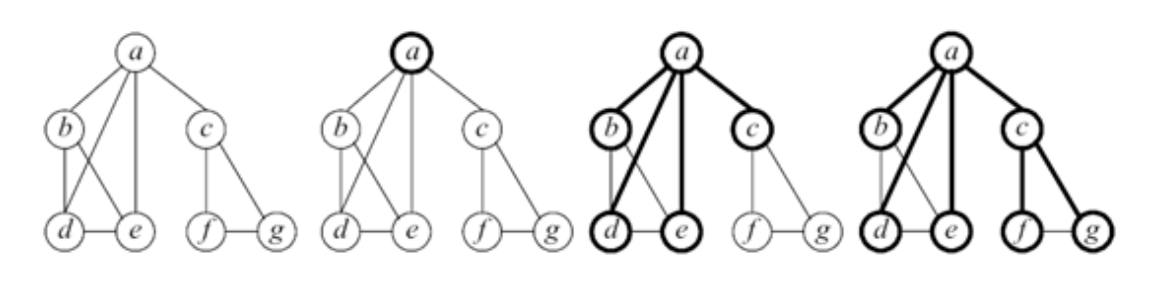
\includegraphics[width=\textwidth]{5_bfs.png}
\end{figure}

Сложность поиска в ширину при нематричном представлении графа
равна $O(n+m)$, так как рассматриваются все n вершин и m ребер.
Использование матрицы смежности приводит к оценке $O(n^2)$.

Если граф не является связным, то нужно добавить шаг 5, в
котором написать, что нужно повторять 2 шаг до тех пор, пока в графе не
останется белых вершин.

Если сначала присвоить первой вершине значение 0, потом
смежным с ней вершинам 0+1 =1, и так далее, то в итоге для каждой
вершины будет найдено расстояние от первой вершины.
\newpage

\begin{definition}
    Поиск в глубину (DFS) исследует конкретную ветку в графе и только потом переходит к другой (если они остануться нерассмотренными).
\end{definition}

Вершины графа могут быть раскрашены в три цвета: белый цвет означает, что
в вершине еще не были, серый – что в вершине были, но еще вернемся, черный
– что были и больше не рассматриваем.

Алгоритм поиска в глубину:
\begin{enumerate}[left=0.0em, labelsep=1em, topsep=0em, itemsep=0pt, parsep=0.5em]
    \item Всем вершинам графа присваиваем белый цвет.
    \item Выбираем первую вершину и раскрашиваем в серый цвет.
    \item Для последней раскрашенной в серый цвет вершины выбираем белую
    смежную ей вершину (если такая вершина есть), раскрашиваем ее в серый цвет
    и переходим к шагу 3.
    \item Повторяем шаг 3 до тех пор, пока все вершины не будут раскрашены в
    черный цвет.
\end{enumerate}

Если для рассматриваемой вершины белых смежных с ней вершин нет, то
рассматриваемую вершину раскрашиваем в черный цвет и переходим к шагу
3.

\begin{figure}[h]
    \centering
    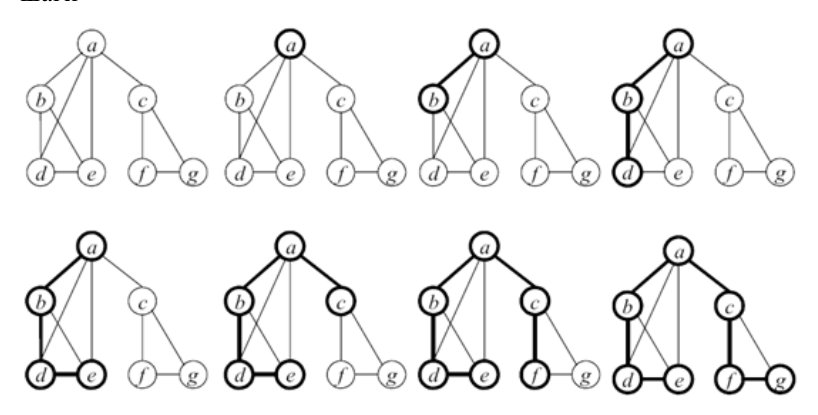
\includegraphics[width=\textwidth]{5_dfs.png}
\end{figure}

Временная сложность алгоритма зависит от представления графа. Если
применена матрица смежности, то временная сложность равна $O(n^2)$, а если
нематричное представление -- $O(n+m)$: рассматриваются все вершины и все ребра.